\documentclass[10pt]{book}
\usepackage[utf8]{inputenc}
\usepackage[italian]{babel}
\usepackage{multicol}
\usepackage[bookmarks]{hyperref}
\usepackage[a4paper, total={18cm, 25cm}]{geometry}
\usepackage{color}
\definecolor{mygray}{rgb}{0.5,0.5,0.5}
\usepackage{listings}
\lstset{
	language=Python,
	commentstyle=\color{mygray},
	morekeywords={function, returns, static, persistent}
}
\usepackage{graphicx}
\usepackage{makecell}
\graphicspath{ {./img/} }
\usepackage{color}

\begin{document}
\renewcommand*\contentsname{Indice}
\title{Introduzione all'Intelligenza Artificiale}
\author{Federico Matteoni}
\date{A.A. 2019/20}
\maketitle
\tableofcontents
\pagebreak
\section*{Introduzione}
Alessio Micheli, Maria Simi\\
\texttt{elearning.di.unipi.it/course/view.php?id=174}\\
Intelligenza Artificiale si occupa della \textbf{comprensione} e della \textbf{riproduzione} del comportamento \textit{intelligente}.\\
Psicologia cognitiva: obiettivo comprensione intelligenza umana, costruendo modelli computazionali e verifica sperimentale.\\
Approccio costruttivo: costruire entità dotate di intelligenze e \textbf{razionalità}. Questo tramite codifica del pensiero razionale per risolvere problemi che richiedono intelligenza non necessariamente facendolo come lo fa l'uomo.\\
Definizioni di IA: pensiero-azione, umanamente-razionalmente.\\
Costruire macchine intelligenti sia che operino come l'uomo che diversamente.\\
formalizzaz conoscenze e meccanizzazione ragionemtno in tutti i settori dell'uomo\\
comprensione tramite modelli comp della psicologia e comportamente di uomini, animali ecc\\
rendere il lavoro con il calcolatore altrettanto facile e utile che del lavoro con persone capaci, abili e disponibili.\\\\
Poniamo definizione di IA: arte di creare macchine che svolgono funzioni che richiedono intelligenza quando svolte da esseri umani. Non definisce "Intelligenza", cosa significa "intelligente"?\\

\chapter{Agenti Intelligenti}
\section{Intelligenza}
L'intelligenza è vista come l'avere diverse capacità, durante il progresso nell'area di ricerca: buon senso, interazione con un ambiente, acquisizione di esperienza, comunicazione, ragionamento logico\ldots
\paragraph{Considerazioni} L'intelligenza quindi non è una collezione di tecniche per risolvere problemi \textbf{specifici}, ma per l'informatica consiste nel \textbf{fornire metodologie sistematiche per dotare le macchine di comportamenti intelligenti/\textit{razionali} su problemi generali \textit{difficili}}.
\section{Agenti}
Iniziamo con inquadrare gli \textbf{agenti}. L'approccio moderno dell'IA consiste della costruzione di agenti intelligenti. Questa visione ci offre un quadro di riferimento ed una prospettiva \textbf{diversa} all'analisi dei sistemi software.\\
Il primo obiettivo sarà di costruire agenti per la risoluzione di problemi vista come una \textbf{ricerca in uno spazio di stati} (\textbf{problem solving})
\begin{center}
	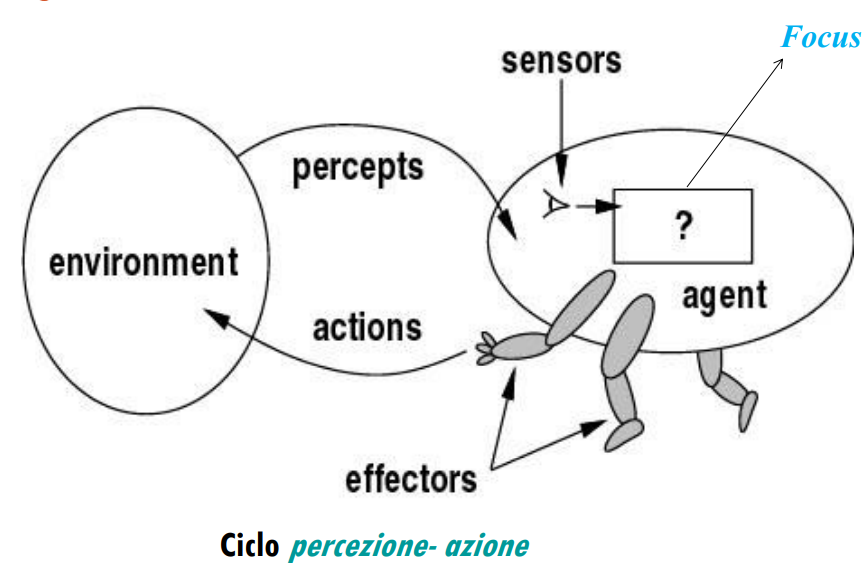
\includegraphics[scale=0.7]{agenti.png}
\end{center}
\subsection{Caratteristiche}
Sono qualcosa di più di un modulo software.
\paragraph{Situati} Gli agenti sono \textbf{situati in un ambiente} da cui \textbf{ricevono percezioni} e su cui \textbf{agiscono} mediante \textbf{azioni} (\textbf{attuatori}).
\paragraph{Sociali} Gli agenti hanno \textbf{abilità sociali}: comunicano, collaborano e si difendono da altri agenti.
\paragraph{Credenze, obiettivi, intenzioni\ldots}
\paragraph{Corpo} Gli agenti hanno un \textbf{corpo}, sono \textbf{embodied} fino a considerare i meccanismi delle emozioni.
\subsection{Percezioni e Azioni}
\paragraph{Percezione} Una percezione è un input da sensori.
\paragraph{Sequenza percettiva} Storia \textbf{completa} delle percezioni\\
La \textbf{scelta delle azioni} è \textbf{unicamente determinata dalla sequenza percettiva}.
\paragraph{Funzione Agente} Definisce l'azione da intraprendere per ogni sequenza percettiva e \textbf{descrive completamente l'agente}. Implementata da un \textbf{programma agente}.
\begin{center}
	\textbf{Sequenza Percettiva} $\longrightarrow^f$ \textbf{Azione}
\end{center}
Il compito dell'IA è progettare il programma agente.
\subsection{Agente e ambiente}
\paragraph{Architettura astratta}
\begin{center}
	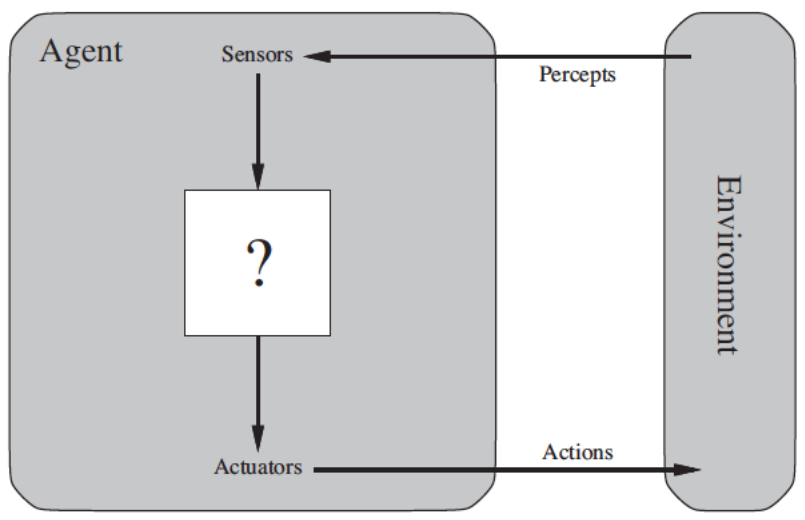
\includegraphics[scale=0.7]{ambiente.png}
\end{center}
\paragraph{Esempi}
\begin{list}{}{}
	\item \textbf{Agente robotico} Percepisce con camera, microfoni e sensori. Interagisce con motori, voce\ldots
	\item \textbf{Agente finanziario} Percepisce i tassi, le news. Interagisce con acquisti e scambi.
	\item \textbf{Agente di gioco} Percepisce le mosse dell'avversario. Interagisce tramite le proprie mosse.
	\item \textbf{Agente diagnostico} Percepisce i sintomi e le analisi dei pazienti. Interagisce fornendo la diagnosi.
	\item \textbf{Agente web} Percepisce le query utente e le pagine web. Interagisce fornendo i risultati di ricerca.
\end{list}
\subsection{Agenti Razionali}
\paragraph{Agenti razionali} Un agente razionale \textbf{interagisce con l'ambiente in maniera efficace}: "\textit{fa la cosa giusta}". L'agente razionale raggiunge l'obiettivo nella maniera più efficiente.\\
Serve quindi una \textbf{misura di prestazione}, di \textit{come vogliamo che il mondo evolva}, a seconda del problema e considerato l'ambiente.
\begin{list}{}{}
	\item \textbf{Esterna}, perché bisogna definirla \textit{prima} di agire. Non si può definire l'obiettivo dopo aver iniziato ad agire, altrimenti non è significativo.\\
	Esempio: la volpe che non arriva all'uva.
	\item Scelta dal progettista a seconda del problema e considerando l'effetto che ha sull'ambiente.
\end{list}
\paragraph{Razionalità} La razionalità è relativa/dipende da:
\begin{list}{}{}
	\item Misura delle prestazioni
	\item Conoscenze pregresse dell'ambiente
	\item Percezioni presenti e passate (sequenza percettiva)
	\item Capacità dell'agente (le azioni possibili)
\end{list}
\paragraph{Definizione} Un \textbf{agente razionale}, quindi, \textbf{esegue l'azione che massimizza il valore atteso della misura delle prestazioni per ogni sequenza di percezioni}, considerando le sue percezioni passate e la sua conoscenza pregressa.\\
Non si pretende perfezione e conoscenza del futuro, ma massimizzare il risultato \textit{atteso}. Potrebbero essere necessarie azioni di acquisizione di informazioni o esplorative (\textbf{non onniscenza}).\\
Le capacità dell'agente possono essere limitate (\textbf{non onnipotenza}).
%https://elearning.di.unipi.it/pluginfile.php/30315/mod_resource/content/0/2-2020-agents.pdf, 22 da fare raz e apprendimento
\paragraph{Agenti autonomi} nella misura in cui il suo comportamento dipende dalla sua esperienza
\paragraph{PEAS} Prestazioni, Environment, Attuatori, Sensori.
\paragraph{Esempio guidatore di taxi} \ldots
\paragraph{Proprietà Ambiente-Problema} Completamenteo/parzialmente osservabile, agente/multi agente, deterministico/stocastico, episodico/sequenziale, statico/dinamico, discreto/continuo, noto/ignoto
\paragraph{Simulatore di ambienti}
\paragraph{Proprietà degli ambienti}
\paragraph{Strutture di agenti caratteristici}
\paragraph{Architettura} Architettura, un corpo e il \textbf{programma}. Ag: P $\longrightarrow$ ...
\paragraph{Agente reattivo semplice} Programma contiene le condizioni azioni. in base a stato interno e regola fornisce la regola da prendere e con la sua azione agisco.
\paragraph{Agenti con obiettivo}
\paragraph{Agenti che apprendono}
\ldots\\
\ldots\\
determinare obiettio e formulare il problema è tanta intelligenza, spostata sull'umano in fase di design. Gli algoritmi sono ancora stupidi.\\
assunzioni\\
stati impliciti perché tanti, quindi vengono fuori in fase di elaborazione e di sviluppo delle decisioni.\\

\end{document}
